\documentclass[xcolor=dvipsnames]{beamer}
% Sandpiles
\mode<presentation>
\usetheme{silab} 
\usecolortheme{silab}

\usepackage{listings}
\usepackage{pxfonts}

% Show Date in title
\def\showtitledate{}
%\def\fancystyle{}
%\def\showshorttitle{}


% Some color definitions
\definecolor{mygray}{gray}{.75}
\definecolor{titlegray}{gray}{.35}
\definecolor{lightgray}{gray}{.85}
\definecolor{topgray}{gray}{.85}
\definecolor{myblue}{rgb}{0.8, 0.85, 1}
\definecolor{topblue}{rgb}{0.68, 0.68, 0.88}
\definecolor{visblack}{rgb}{0.0, 0.0, 0.0}

% Boxes
\setbeamercolor{uppercol}{fg=black,bg=myblue}
\setbeamercolor{lowercol}{fg=black,bg=mygray}

\usepackage[english]{babel}
\usepackage[utf8]{inputenc}
\usepackage[T1]{fontenc}
\usepackage{graphicx}
\usepackage{amsmath,commath,amsfonts,amssymb,mathtools}
\usepackage{pgf}
\usepackage[autostyle=true]{csquotes}
\usepackage{IEEEtrantools}
\usepackage[varg]{txfonts}
\usepackage{hyperref}
\usepackage{xcolor}
\usepackage{siunitx}
\usepackage{fancyhdr}
\usepackage{colortbl}
\usepackage{geometry}
\usepackage{caption}
\usepackage{siunitx}
\usepackage{verbatim}
\usepackage{subfigure}
\usepackage{booktabs}
\usepackage{empheq}
\usepackage{animate}
\usepackage{float}
\usepackage{pdfpages}
\usepackage{floatflt}
\usepackage{overpic}
\usepackage{scalerel}
\usepackage{tikz}
\graphicspath{{./pics/}{./gifs/}{../analysis/avalanche_formations/}{../analysis/moment_analysis/plots/}{../analysis/naive_fits/}}
%\usepackage{ubonn-biblatex}
\usepackage[sorting=none, natbib=true, style=numeric]{biblatex}


\addto{\captionsenglish}{\renewcommand*{\figurename}{Fig.}}
\setbeamertemplate{caption}[numbered]

\newcommand*\widefbox[1]{\fbox{\hspace{2em}#1\hspace{2em}}}
\newcommand{\myitemsep}{\setlength\itemsep{0.33cm}}
\newcommand{\mysubitemsep}{\setlength\itemsep{0.22cm}}

\newcommand{\backupbegin}{
	\newcounter{finalframe}
	\setcounter{finalframe}{\value{framenumber}}
}
\newcommand{\backupend}{
	\setcounter{framenumber}{\value{finalframe}}
}

% Coding stuff
\lstset{language=python, numbers=left, numberstyle=\tiny, showstringspaces=false,
	aboveskip=10pt, frame=leftline}

% No stupid navigation bar
\beamertemplatenavigationsymbolsempty

\useinnertheme{rectangles}
%\setbeamertemplate{navigation symbols}{}

\title[Sandpiles]{Cellular Automata for Sandpiles}
\author[M. Frohne \& P. Wolf]{Markus Frohne\\ \texttt{\textcolor{gray}{markusfrohne@uni-bonn.de}}\\ \vspace{0.33cm} Pascal Wolf\\ \texttt{\textcolor{gray}{pwolf@uni-bonn.de}}}
\date{March 15$^\text{th}$, 2018}

\addbibresource{../report/refs.bib}

\newcommand{\fplus}[1][black]{%
	\tikz\draw[#1,line width=2pt] (0,0) -- (0.25,0)(0.125,0.125) -- (0.125,-0.125);
}

\newcommand{\fminus}[1][black]{%
	\tikz\draw[#1,line width=2pt] (0,0) -- (0.25,0);
}

\begin{document}
	
	\begin{frame}
		\titlepage
	\end{frame}
	
	\begin{frame}{Outline of talk}
		\begin{itemize}
			\myitemsep
			\item {Introduction:
				\vspace{0.22cm}
				\begin{itemize}
					\mysubitemsep
					\item[$\bullet$] Motivation
					\item[$\bullet$] Self-organized criticality (\textbf{SOC})
				\end{itemize}
				}
			\item {Theory and simulation:
				\vspace{0.22cm}
				\begin{itemize}
					\mysubitemsep
					\item[$\bullet$] Cellular automata for sandpile dynamics: The \texttt{Bak-Tang-Wiesenfeld} (\textbf{BTW}) and custom model
				\end{itemize}}
			\item Analysis
			\item {Results
				\vspace{0.22cm}
				\begin{itemize}
					\mysubitemsep
					\item[$\bullet$] Discussion
					\item[$\bullet$] Comparison of models
				\end{itemize}}
			\item Summary
		\end{itemize}
	\end{frame}
	
	{\usebackgroundtemplate%
		{%
			
\includegraphics[width=\paperwidth,height=\paperheight]{bkg1.pdf}%
		}
		\begin{frame}
			\centering \Huge \color{ublue} Introduction
			\thispagestyle{empty}
			\addtocounter{framenumber}{-1}
		\end{frame}
	}
	
	{\usebackgroundtemplate%
		{%
			
\includegraphics[width=\paperwidth,height=\paperheight]{bkg1.pdf}%
		}
		\begin{frame}
			\centering \Huge \color{ublue} Simulation results and analysis
			\thispagestyle{empty}
			\addtocounter{framenumber}{-1}
		\end{frame}
	}
	
	\begin{frame}{Sandpile dynamics -- Avalanche evolution}
		\begin{figure}[h]
			\captionsetup{width=0.9\textwidth}
			\centering
			\only<1>{
			\subfigure[BTW model]{\animategraphics[width=0.475\textwidth, loop, autoplay]{10}{btw_random_}{1}{250}}
			\subfigure[Custom model]{\animategraphics[width=0.475\textwidth, loop, autoplay]{10}{custom_random_}{1}{250}}
			\caption{Avalanche evolution in a 2D sandbox of length 50 (\textbf{random} drives)}}
			\only<2>{
			\subfigure[BTW model]{\animategraphics[width=0.475\textwidth, loop, autoplay]{10}{btw_center_}{1}{250}}
			\subfigure[Custom model]{\animategraphics[width=0.475\textwidth, loop, autoplay]{10}{custom_center_}{1}{250}}
			\caption{Avalanche evolution in a 2D sandbox of length 50 (\textbf{center} drives)}}
		\end{figure}
	\end{frame}
	
	\begin{frame}{Sandpile dynamics -- Avalanche formation}
		\begin{figure}[h]
			\captionsetup{width=0.9\textwidth}
			\begin{center}
				\only<1>{
				\subfigure[2D]{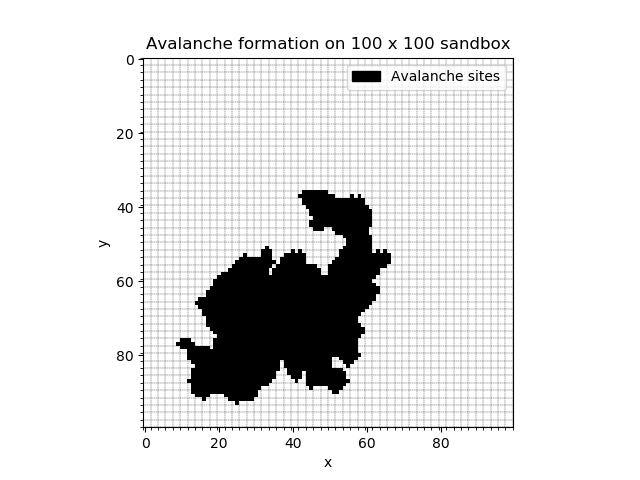
\includegraphics[width=0.475\textwidth]{Avalanche_2d_btw_1.png}}
				\subfigure[3D]{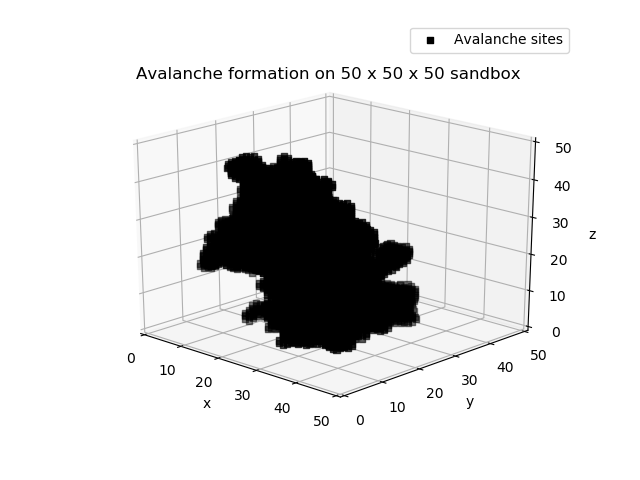
\includegraphics[width=0.475\textwidth]{Avalanche_3d_btw_6.png}}
				\caption{Avalanche formation in the BTW model.}}
				\only<2>{
				\subfigure[2 D]{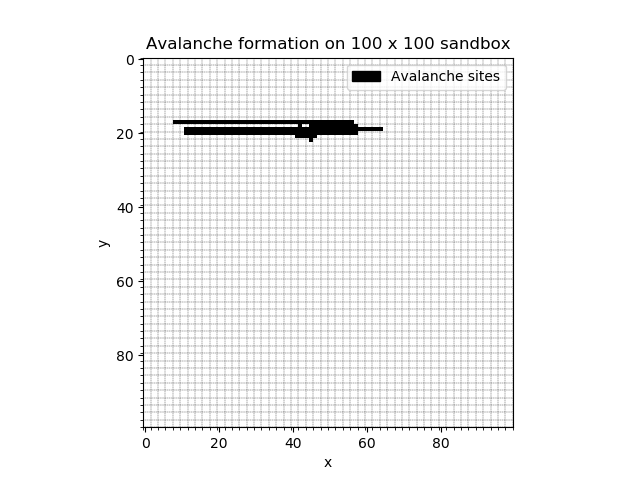
\includegraphics[width=0.475\textwidth]{Avalanche_2d_custom_11.png}}
				\subfigure[3 D]{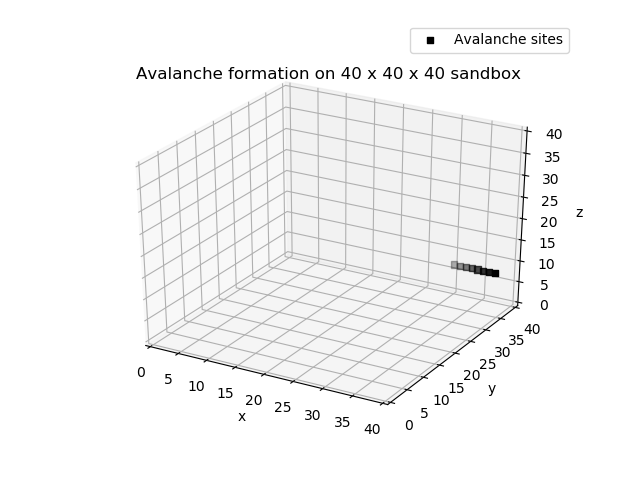
\includegraphics[width=0.475\textwidth]{Avalanche_3d_custom_4.png}}
				\caption{Avalanche formation in the custom model.}}
			\end{center}
		\end{figure}
	\end{frame}
	
	\begin{frame}{Sandpile dynamics -- Power law scaling}
		\begin{figure}[h]
			\captionsetup{width=0.9\textwidth}
			\begin{center}
				\subfigure[Duration]{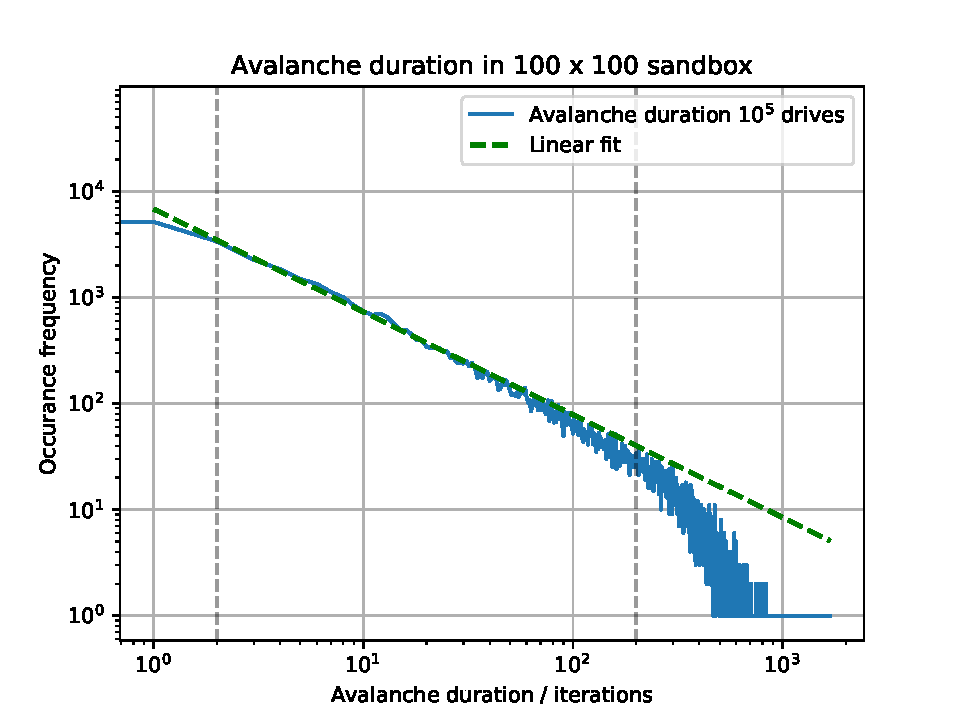
\includegraphics[width=0.45\textwidth]{naive_fit.pdf}}
				\subfigure[Size]{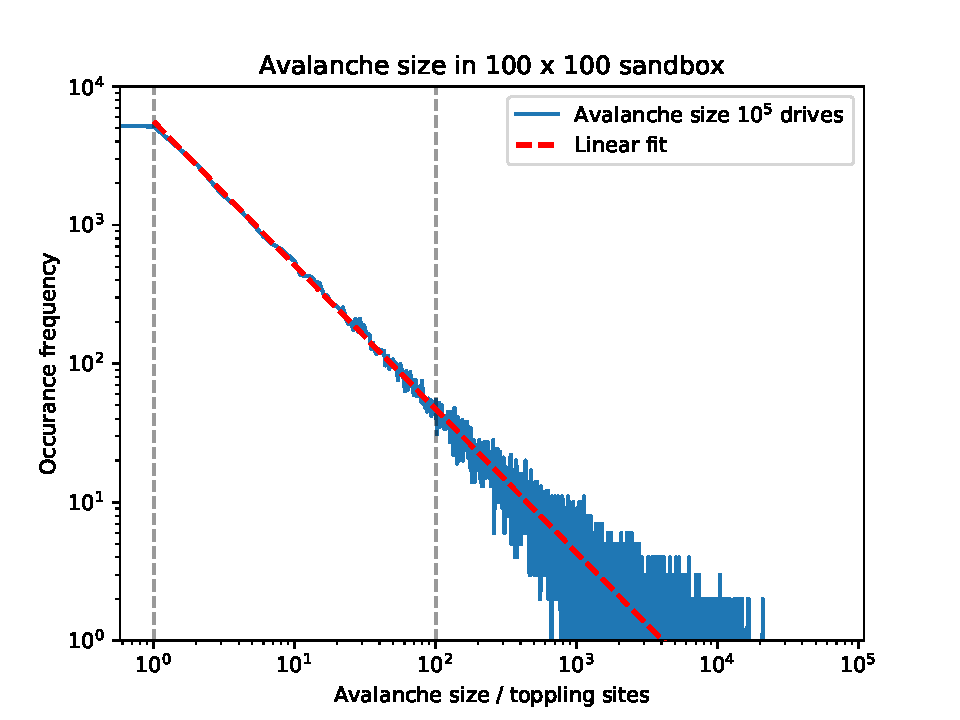
\includegraphics[width=0.45\textwidth]{naive_fit2.pdf}}
				\caption{Power law scaling behavior of avalanche duration and size of the BTW model.}
			\end{center}
		\end{figure}
	\end{frame}
	
	\begin{frame}{Sandpile dynamics -- Moment analysis}
		\begin{itemize}
			\myitemsep
			\item {Define the so-called $n^{\mathrm{th}}$ \textit{moment} of the observable $y$ by
				\begin{align*}
				\left\langle y^n \right\rangle := \int_{0}^{\infty} dy y^n P^{(y)}(y)
				\end{align*}
				where $P^{(y)}$ is the PDF of $y$.
				}
			\item {For $\lim{L \to \infty}$ the following relation holds:
				\begin{align*}
				\left\langle y^n \right\rangle \propto L^{K\left(1 + n - \rho \right)} \qquad \text{with} \qquad K\left(1 + n - \rho \right) \equiv \sigma_n 
				\end{align*}
				where  $K,\ \rho$ is the \textbf{set of critical exponents} of the observable $y$. Taking the logarithm, this relation exhibits a linear trend with slope $\sigma_n$.
				}
			\item {Determination exponents of the $1^{\text{st}}$ and $2^{\text{nd}}$ moment $\sigma_1$ and $\sigma_2$ allows for the calculation of the set of critical exponents $K,\ \rho$:
				\begin{align*}
				K = \sigma_2 - \sigma_1 \quad , \quad \rho = \frac{2\sigma_2 - 3\sigma_1}{\sigma_2 - \sigma_1} 
				\end{align*} 
				}
		\end{itemize}
	\end{frame}
	
	\begin{frame}{Sandpile dynamics -- Moment analysis}
		\begin{itemize}
			\myitemsep
			\item[$\Rightarrow$] Simulate $N$ samples of $O$ and calculate the critical exponents $D,\ \rho$ within several \textit{bootstraps} to estimate their numerical value as well as standard deviation from it.
		\end{itemize}
	\end{frame}
		
\end{document}